% To je predloga za poročila o domačih nalogah pri predmetih, katerih
% nosilec je Blaž Zupan. Seveda lahko tudi dodaš kakšen nov, zanimiv
% in uporaben element, ki ga v tej predlogi (še) ni. Več o LaTeX-u izveš na
% spletu, na primer na http://tobi.oetiker.ch/lshort/lshort.pdf.
%
% To predlogo lahko spremeniš v PDF dokument s pomočjo programa
% pdflatex, ki je del standardne instalacije LaTeX programov.

\documentclass[a4paper,11pt]{article}
\usepackage{a4wide}
\usepackage{fullpage}
\usepackage[utf8x]{inputenc}
\usepackage[slovene]{babel}
\selectlanguage{slovene}
\usepackage[toc,page]{appendix}
\usepackage[pdftex]{graphicx} % za slike
\usepackage{setspace}
\usepackage{color}
\definecolor{light-gray}{gray}{0.95}
\usepackage{listings} % za vključevanje kode
\usepackage{hyperref}
\usepackage{amsmath}
\usepackage{amssymb}
\usepackage{caption}
\usepackage{subcaption}
\renewcommand{\baselinestretch}{1.2} % za boljšo berljivost večji razmak
\renewcommand{\appendixpagename}{Priloge}

\lstset{ % nastavitve za izpis kode, sem lahko tudi kaj dodaš/spremeniš
language=Python,
basicstyle=\footnotesize,
basicstyle=\ttfamily\footnotesize\setstretch{1},
backgroundcolor=\color{light-gray},
}

\title{Detekcija ključnih točk}
\author{David Rubin (david.rubin@student.um.si)}
\date{\today}

\begin{document}

\maketitle

\section{Zahteve naloge}

Za poročilo/zagovor se pričakujejo naslednje demonstracije:
\begin{itemize}
    \item \textbf{Fast detektor}
        \begin{itemize}
        	\item hiter test \\
            Na sliki prikažite točke, ki jih potrdite s hitrim testom in točke, ki jih potrdite s celotnim testom. Za izbrano testno sliko preštejte in primerjajte število točk najdenih s hitrim testom z številom končnih točk.
        \item odstranjevanje nemaksimalnih odzivov \\
            Prikažite točke pred in po odstranjevanju nemaksimalnih odzivov.
        \item iskanje točk različnih velikosti \\
            Točke različnih velikosti ločeno prikažite na izvorni sliki. Prikažite rezulatate za vsaj tri velikosti.

          \end{itemize}
            \item \textbf{BRIEF deskriptor}
            \begin{itemize}
            
        \item izračun orientacije točke \\
            Za vsako FAST točko v sliki s črto prikažite orientacijo točke (črta je vektor smeri). Prikažite tudi rezultate za isto sliko, rotirano za 45 stopinj na kateri bodo vidne iste točke z ustrezno prilagojenimi orientacijami.
        \item izračun orientacije opisa \\
            Za FAST točko v sliki izrišite izbrane BRIEF točke v njeni okolici (nekje 10 BRIEF točk). Prikažite iste točke poravnane z orientacijo točke v rahlo rotirani sliki (pozicije BRIEF točke bi se morale ohraniti relativno na orientacijo FAST točke).
        \item primerjava točk \\
            Pokažite ujemajoče točke med sliko in njeno rahlo modificirano (translirano, rotirano, skalirano) različico. Večina točk se mora ustrezno ujemati
            \end{itemize}
\end{itemize}

\section{Implementacija}

Nalogo sem implementiral v programsken jeziku Python, za delovanje so potrebne knjižnice \textit{numpy} (za pospešene operacije nad seznami), \textit{matplotlib} (za pomoč pri risanju grafov in slik), in \textit{open-cv} (za branje in pisanje slik). Pri risanju ujemajočih točk med dvema slikama sem še uporabil funkcijo \textit{plot\_matches} iz knjižnice \textit{scikit-image}.
Projekt je sestavljen iz 4 datotek:
\begin{itemize}
	\item \texttt{fast.py} vsebuje implementacijo detektorja ključnih točk FAST,
	\item \texttt{brief.py} vsebuje implemetacijo deskriptorja BRIEF,
	\item \texttt{orb.py} povezuje prej omenjeni datoteki in nudi metodo, ki skuša povezati ključne točke na 2 \textit{podobnih} slikah,
	\item \texttt{utils.py} pa vsebuje pomožne metode, kot so recimo izračun Hammingove razdalje ali pa branje slik iz datotek.
\end{itemize}

Za demonstracijo delovanja algoritma FAST smo uporabili sliko~\ref{img:blox}.

\begin{figure}[hbp]
	\centering
	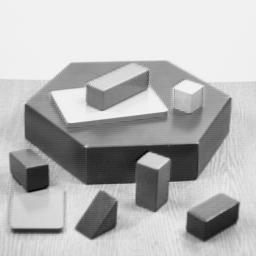
\includegraphics[width=0.7\textwidth]{images/blox}
	\caption{Slika blox. \small Vir: http://52.55.172.202/testes/opencv-3.2.0/samples/data/}
	\label{img:blox}
\end{figure}

\subsection{Hitri test vs. poln}
Pri hitrem testu preverjam le 4 skrajne točke v krogu okoli opazovanega oglišča (skrajno severno, južno, vzodno in zahodno). Kadar so vrednosti v vsaj 3 izmed teh ogliščih višje oziroma nižje od praga. Torej veljati mora
\begin{equation}
\begin{gathered}
	p_x > p_{center} + t \\
	\text{ali} \\
	p_x < p_{center} - t, \\
\end{gathered}
\label{eq:corner_condition}
\end{equation}
pri čemer $p_x$ predstavlja vrednost piksla v enem izmed 4 pozicij, $p_{center}$ predstavlja opazovan piksel (kandidat za ključno točko), $t$ pa je uporabniško določena pragovna vrednost.
V kolikor je hitri test pokazal morebitno ogljišče nad to lokacijo preverim še vseh 16 pikslov, ki jo obkrožajo, pri temu pa mora veljati, da je vsaj 12 zaporednih, ki ustrezajo (izključno) enemu izmed pogojev~\ref{eq:corner_condition}.

Nad testno sliko~\ref{img:blox} je bila pognana priložena implementacija FAST algoritma s pragovno vrednostjo 17 in brez odstranjevanja kandidatov s pomočjo nemaksimalnih odzivov (angl. \textit{nonmax supression}). Rezultati so vidni na sliki~\ref{img:kp_speed_comparison}.

\begin{figure}[hb]
	\centering
	\begin{subfigure}[t]{0.48\textwidth}
		\centering
		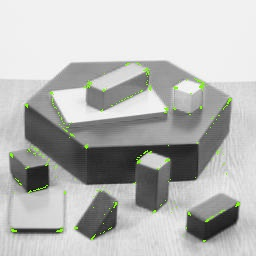
\includegraphics[width=\textwidth]{images/blox_corners_high-speed.jpg}
		\caption{Kandidati za ključne točke (oglišča) pridobljeni s pomočjo hitrega testa.}
		\label{img:kp_high_speed}
	\end{subfigure}
	\hfill
	\begin{subfigure}[t]{0.48\textwidth}
		\centering
		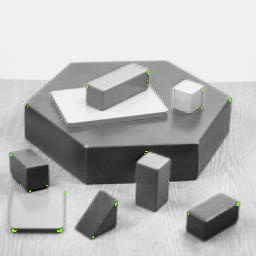
\includegraphics[width=\textwidth]{images/blox_corners_all.jpg}
		\caption{Ključne točke, ki smo jih potrdili kot oglišča.}
		\label{img:kp_high_speed}
	\end{subfigure}
	\caption{Ključne točke so označene z zeleno barvo. Pragovna vrednost je znašala 17 in opcija nonmax je bila izključena (\texttt{False}).}
	\label{img:kp_speed_comparison}
\end{figure}

\subsection{Odstranjevanje nemaksimalnih odzivov}

Pri odstranjevanju nemaksimalnih odzivov skušamo omejiti vpliv pikslov, ki so blizu skupaj in sklepamo, da opisujejo isto ogljišče. Za vsako ključno točko poračunamo vrednost:
\begin{equation}
	\begin{gathered}
	s = \sum_{n=1}^{16}{p_n - p_{center} - t} \\
	\text{oziroma} \\
	s = \sum_{n=1}^{16}{p_{center} - t - p_n}
	\end{gathered}
\end{equation}
Pri tem predstavlja $p_{center}$ pikselno vrednost v središču, $t$ je pragovna vrednost, $p_n$ pa vrednost na krožnici okoli centra.
Prva enačba velja, kadar smatramo ključtno točko svetlejšo od pragovne vrednosti, druga pa kadar je temnejša. V kolikor imamo takšno vrednost, lahko za vsako ključno točko preverimo sosednje piksle in odstranimo tiste, ki imajo nižjo vrednost. Rezultat primerjave detekcije točk z uporabe te tehnike in brez je predstavljen na sliki~\ref{img:kp_nonmax_comparison}.

\begin{figure}[hb]
	\centering
	\begin{subfigure}[t]{0.48\textwidth}
		\centering
		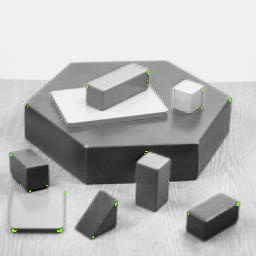
\includegraphics[width=\textwidth]{images/blox_corners_all.jpg}
		\caption{Ogljišča brez uporabe nonmax.}
		\label{img:kp_wo_nonmax}
	\end{subfigure}
	\hfill
	\begin{subfigure}[t]{0.48\textwidth}
		\centering
		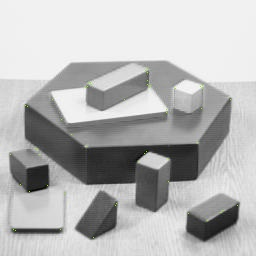
\includegraphics[width=\textwidth]{images/blox_corners_nmax.jpg}
		\caption{Ogljišča po uporabi nonmax.}
		\label{img:kp_w_nonmax}
	\end{subfigure}
	\caption{Piksli ključnih točk so označene z zeleno barvo. Pragovna vrednost je znašala 17.}
	\label{img:kp_nonmax_comparison}
\end{figure}

\subsection{Točke različnih velikosti}

Pri iskanju oglišč v različnih velikostih sem vpleljal piramido slik, torej izvorno sliko pomanjšamo (v mojem primeru za faktor 2), kar pomeni, da izgubimo delež podrobnosti in posledično lahko iščemo le najizrazitejša ogljišča. Detekcija poteka na vsaki izmed pomanjšanih slik, na katere se tudi vrišejo zaznane ključne točke. Primerjava točk je vidna na sliki~\ref{img:kp_size_comparison}

\begin{figure}[h!b]
	\centering
	\begin{subfigure}[t]{0.48\textwidth}
		\centering
		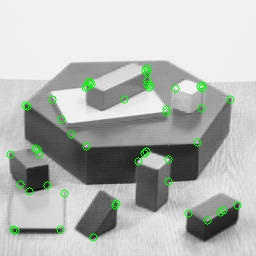
\includegraphics[width=\textwidth]{images/blox_corners_L0.jpg}
		\caption{Ogljišča na izvorni sliki (velikost slike je $256\times256$).}
		\label{img:kp_L0}
	\end{subfigure}
	\hfill
	\begin{subfigure}[t]{0.48\textwidth}
		\centering
		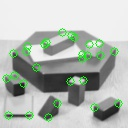
\includegraphics[width=\textwidth]{images/blox_corners_L1.jpg}
		\caption{Ogljišča na prvem podnivoju (velikost slike je $128\times128$).}
		\label{img:kp_L1}
	\end{subfigure}
	\begin{subfigure}[t]{0.48\textwidth}
		\centering
		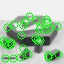
\includegraphics[width=\textwidth]{images/blox_corners_L2.jpg}
		\caption{Ogljišča na drugem podnivoju (velikost slike je $64\times64$).}
		\label{img:kp_L2}
	\end{subfigure}
	\caption{Ključne točke so označene kot zeleni krogci s konstantnim polmerom 4 pikslov. Pragovna vrednost je znašala 17, uporabljen je bil tudi nonmax. Opazimo, da se med sliko \ref{img:kp_L0} in \ref{img:kp_L1} izgubi nekaj ogljišč (izrazitejša obstanejo), slednje pa opazimo tudi med slikama \ref{img:kp_L1} in \ref{img:kp_L2} (npr. zgornji levi kot na belem kvadru).}
	\label{img:kp_size_comparison}
\end{figure}

\clearpage

\subsection{Izračun orientacije točk}

Izračun orientacije točk poteka preko centroida intenzitete (angl. \textit{intensity centroid}), pri čemer skušamo izračunati center intenzitete pikslov v krožnem območju okoli opazovane točke. Vektor smeri označen na slikah je potem daljica iz središča ključne točke do izračunanega centra na območju okoli točke. Na sliki~\ref{img:orientation_comparison} je prikazan primer orientacije ključnih točk zaznanih na rotiranih slikah.
\begin{figure}[hb]
	\centering
	\begin{subfigure}[t]{0.48\textwidth}
		\centering
		
\includegraphics[width=\textwidth]{images/orientations_0.png}
		\caption{Ključne točke in njihove orientacije na testni sliki.}
		\label{img:orientations0}
	\end{subfigure}
	\hfill
	\begin{subfigure}[t]{0.48\textwidth}
		\centering
		
\includegraphics[width=\textwidth]{images/orientations_45.png}
		\caption{Ključne točke in njihove orientacije na isti sliki rotirani za 45 stopinj. }
		\label{img:orientations45}
	\end{subfigure}
	\caption{Primerjava ohranitve orientacije ključnih točk (označene kot zelene puščice) ob rotiranju slike za kot 45 stopinj v obratni smeri urinega kazalca. Orientacije so se ohranile v večini od skupaj zaznanih točk. Uporabili smo okroglo okno velikosti 31 pisklov.}
	\label{img:orientation_comparison}
\end{figure}

\clearpage

\subsection{Izračun orientacije opisa}

Za prikaz orientiranega opisa sem uporabil izrez iz slike šahovskih figur~\ref{img:match_base} in jo večkrat rotiral. Pri obeh slikah sem ročno poiskal ujemajoče ključne točke z algoritmom FAST, in zanje nato poračunal orientacijo nekaj naključnih BRIEF točk. BRIEF točke se generirajo naključno, rezultati dveh zagonov so vidni na slikah~\ref{img:brief_orientation} in~\ref{img:brief_orientation1}.


\begin{figure}[h!b]
	\centering
	\begin{subfigure}[t]{0.48\textwidth}
		\centering
		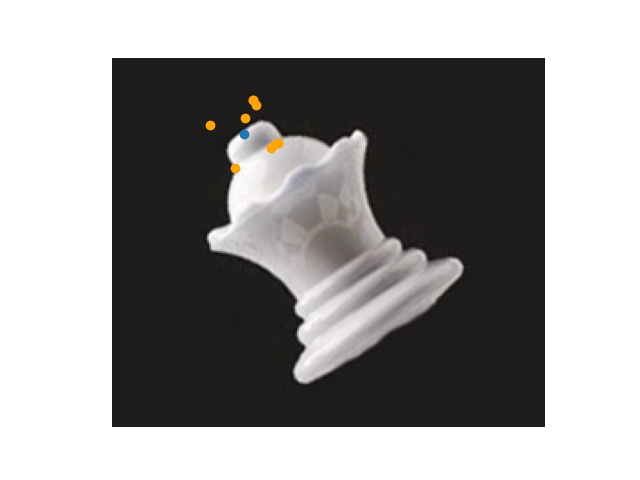
\includegraphics[width=\textwidth]{images/brief_orientation_0.png}
		\caption{Naključne BRIEF točke poravnane glede na orientacijo FAST točke.}
		\label{img:brief_orientation_0}
	\end{subfigure}
	\hfill
	\begin{subfigure}[t]{0.48\textwidth}
		\centering
		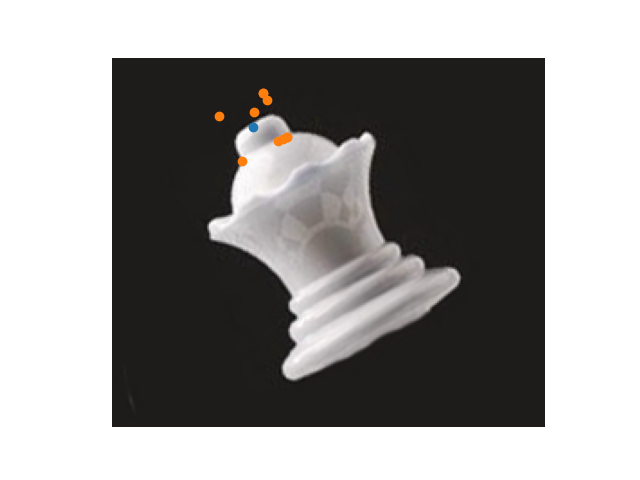
\includegraphics[width=\textwidth]{images/brief_orientation_1.png}
		\caption{Identične BRIEF točke iz slike~\ref{img:brief_orientation_0} poravnane na orientacijo ključne točke v rotirani sliki.}
		\label{img:brief_orientation_1}
	\end{subfigure}
	\caption{Primer naključnih BRIEF točk (obarvane v oranžnem odtenku) poravnanih glede na orientacijo ključne točke (obarvane modro) na izseku vrha dame rotiranega za 30 in 35 stopinj.}
	\label{img:brief_orientation}
\end{figure}

\begin{figure}[h!b]
	\centering
	\begin{subfigure}[t]{0.48\textwidth}
		\centering
		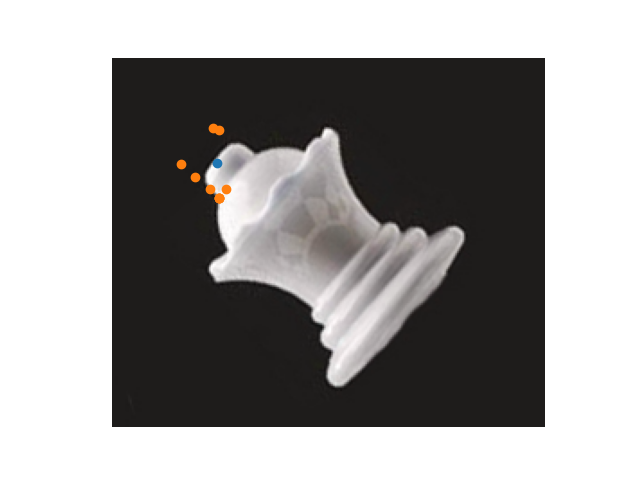
\includegraphics[width=\textwidth]{images/brief_orientation1_0.png}
		\caption{Naključne BRIEF točke poravnane glede na orientacijo FAST točke.}
		\label{img:brief_orientation1_0}
	\end{subfigure}
	\hfill
	\begin{subfigure}[t]{0.48\textwidth}
		\centering
		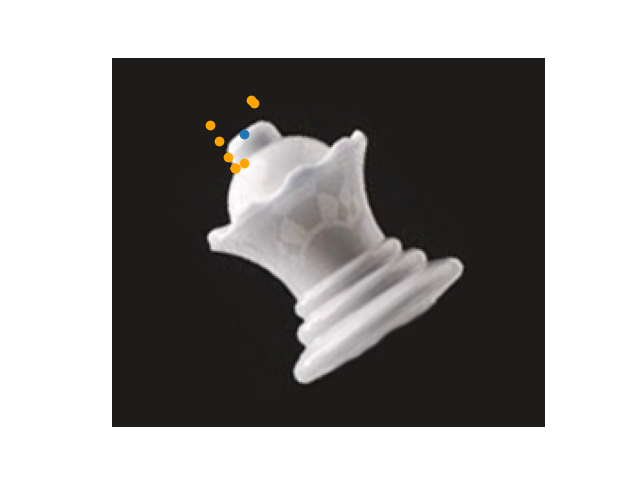
\includegraphics[width=\textwidth]{images/brief_orientation1_1.png}
		\caption{Identične BRIEF točke iz slike~\ref{img:brief_orientation1_0} poravnane na orientacijo ključne točke v rotirani sliki.}
		\label{img:brief_orientation1_1}
	\end{subfigure}
	\caption{Ponoven primer naključnih BRIEF točk (obarvane v oranžnem odtenku) poravnanih glede na orientacijo ključne točke (obarvane modro) izseku vrha dame rotiranega za 30 in 50 stopinj.}
	\label{img:brief_orientation1}
\end{figure}

\clearpage

\subsection{Primerjava točk}

Pri primerjavi točk sem uporabil sliko šahovskih figur~\ref{img:match_base}, iz katere sem nato izrezal odseke z urejevalnikom slik in jih z implementiranim algoritmom ORB skušal umestiti nazaj v izvorno sliko. Za učinkovitejše delovanje je priporočljivo, da se kot prva slika vzame izsek, saj algoritem primerja vsako ključno točko iz prve slike in jih išče najbližjo primerjavo v drugi sliki. Algoritem je prav tako zasnovan, da pri primerjavi točk upošteva prag najvišjega razlikovanja, ki je uporabniško določen. V kolikor najmanjša (Hammingova) razdalja med opazovano ključno točko na prvi sliki in vsemi ključnimi točkami na drugi sliki preseže ta prag, se smatra, da ključna točka nima ustreznega zadetka. Na slikah~\ref{img:match_object},~\ref{img:match_rotate_small} in~\ref{img:match_rotate_scale} so vidni rezultati poskusov. Za vsak poskus so bili uporabljeni parametri: velikost okna 31, velikost deskriptorja 256, FAST prag 25, največja razdalja za ujemanje 35.


\begin{figure}[hb]
	\centering
	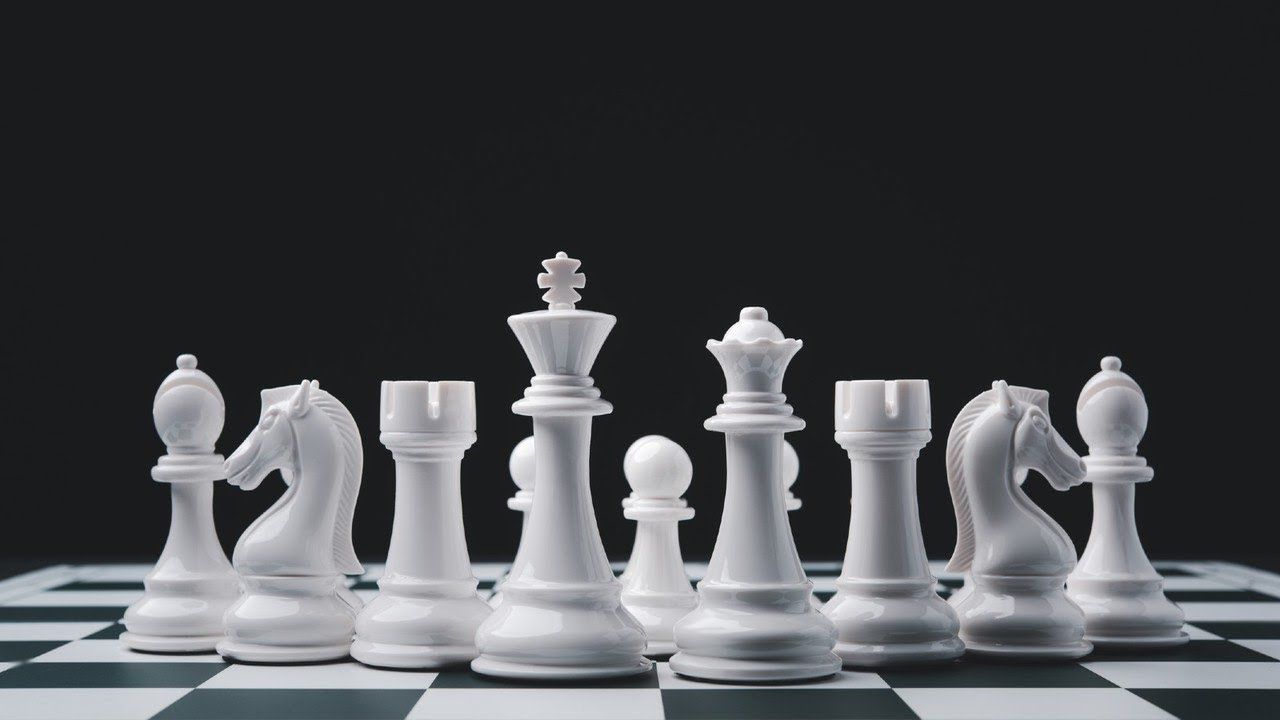
\includegraphics[width=0.8\textwidth]{images/chess.jpg}
	\caption{Slika šahovskih figur, osnova za primerjavo ključnih točk.}
	\label{img:match_base}
\end{figure}

\begin{figure}[hb]
	\centering
	\begin{subfigure}[t]{0.2\textwidth}
		\centering
		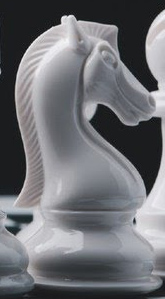
\includegraphics[width=\textwidth]{images/chess-knight.jpg}
		\caption{Izrezan in rotiran vrh kraljevske figure.} 
		\label{img:chess_knight}
	\end{subfigure}
	\begin{subfigure}[t]{1\textwidth}
		\centering
			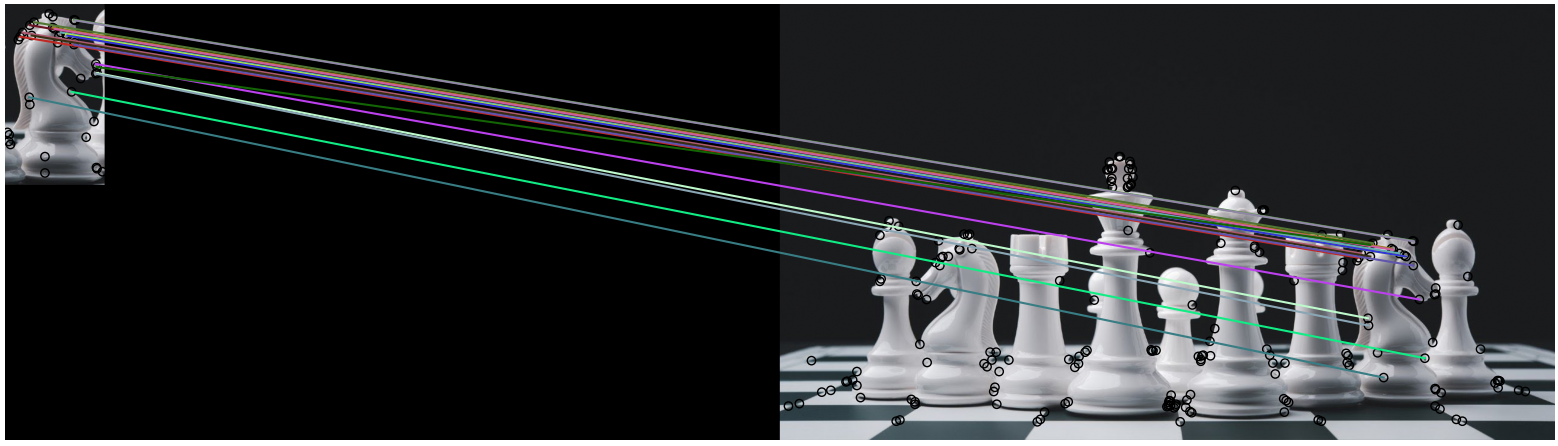
\includegraphics[width=1\textwidth]{images/match_object.png}
		\caption{Ujemanje konja s prvotno sliko.}
		\label{img:chess_knight_match}
	\end{subfigure}
	\caption{Iz prvotne slike izrezan konj in njegovo ujemanje ključnih točk. Ključne točke so se preslikale na isti objekt, vendar z nekoliko zamaknjenimi pozicijami. }
	\label{img:match_object}
\end{figure}


\begin{figure}[hb]
\centering
	\begin{subfigure}[t]{0.48\textwidth}
		\centering
		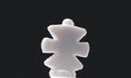
\includegraphics[width=\textwidth]{images/chess_crown.jpg}
		\caption{Izrezan in rotiran vrh kraljevske figure.}
		\label{img:chess_crown}
	\end{subfigure}
	\begin{subfigure}[t]{1\textwidth}
		\centering
			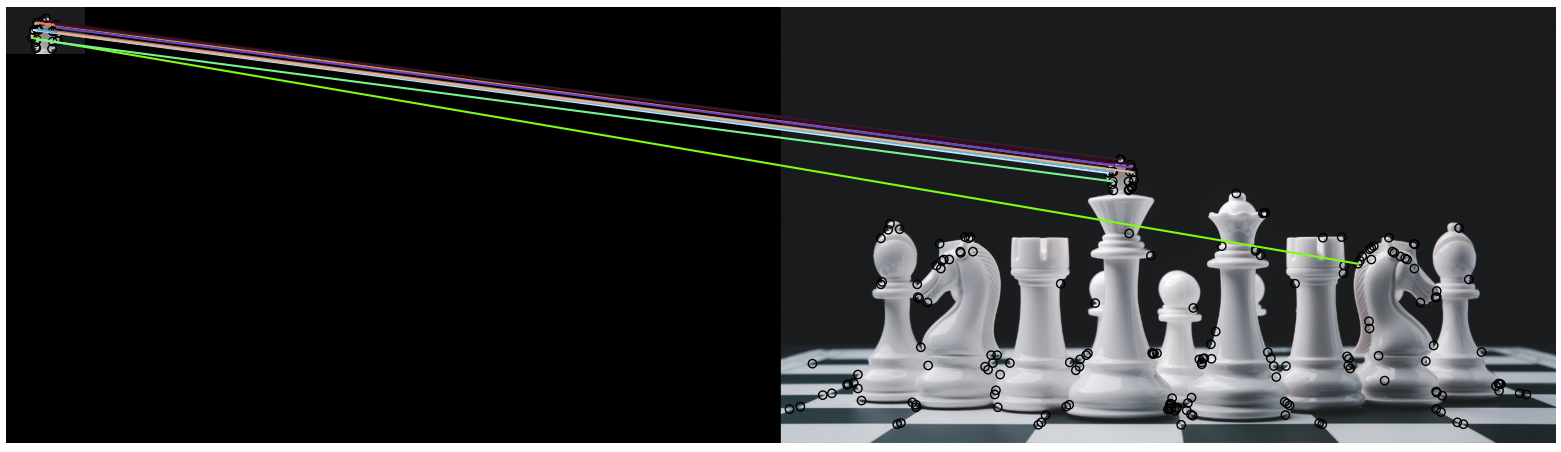
\includegraphics[width=1\textwidth]{images/match_rotate_small.png}
		\caption{Ujemanje modificiranega vrha s prvotno sliko.}
		\label{img:chess_crown_match}
	\end{subfigure}

	\caption{Primerjava ključnih točk na izrezani in malo rotirani kroni iz kraljevske figure. Ena izmed točk se je preslikala na konja, ostale pa so zadele prvotni objekt.}
	\label{img:match_rotate_small}
\end{figure}

\begin{figure}[hb]
\centering
	\begin{subfigure}[t]{0.48\textwidth}
		\centering
		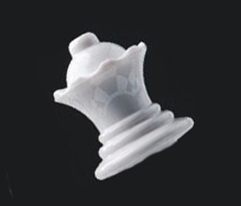
\includegraphics[width=\textwidth]{images/chess_queen.jpg}
		\caption{Izrezan, rotiran in povečan vrh dame.}
		\label{img:chess_queen}
	\end{subfigure}
	\begin{subfigure}[t]{1\textwidth}
		\centering
			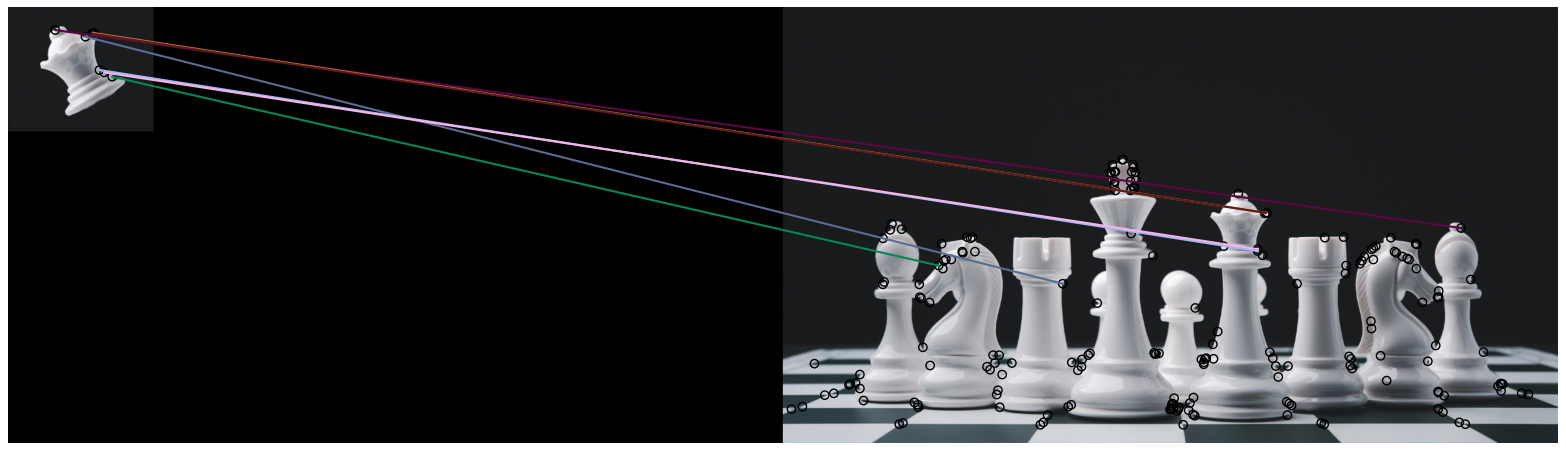
\includegraphics[width=1\textwidth]{images/match_rotate_scale.png}
		\caption{Ujemanje modificiranega vrha s prvotno sliko.}
		\label{img:chess_queen_match}
	\end{subfigure}

	\caption{Primerjava ključnih točk na izrezanem, rotiranem (30 stopinj) in skaliranem (10\% povečava) vrhu dame. Točke so zadele damo, preslikale pa so se tudi na top, tekača in konja. Sklepam, da so ključne točke, ki so se napačno preslikale precej podobne, saj so šahovske figure stilsko usklajene.}
	\label{img:match_rotate_scale}
\end{figure}

\end{document}
